\documentclass{article}
\usepackage{amsmath}  % For mathematical symbols and equations
\usepackage{amsfonts}  % For additional math fonts
\usepackage{graphicx}  % For including graphics
\usepackage{geometry}  % To manage page layout

\geometry{a4paper, margin=1in}  % Set the margins for A4 paper

\title{Computational Modeling of the SIR Disease Model with Hospitalization Dynamics}
\author{Mihai-Alexandru Radu}
\date{September 1, 2024}  % Set the date

\begin{document}

\maketitle  % Generates the title

\begin{abstract}
This paper presents a comprehensive analysis and computational simulation of the SIR (Susceptible, Infected, Recovered) model for epidemic dynamics, incorporating hospitalization effects. Using Python, we derive and solve the relevant ordinary differential equations (ODEs) and analyze the impact of hospitalization on the dynamics of an infectious disease. The model parameters are based on real-world data from the COVID-19 outbreak in Wuhan, China, on January 22, 2020. We provide detailed explanations of the ODE derivations, visualize the results, and discuss the implications of hospitalization on disease spread.
\end{abstract}

\section{Introduction}
The SIR model is a fundamental framework in epidemiology, used to understand the spread of infectious diseases by dividing the population into susceptible, infected, and recovered compartments. This study extends the classic SIR model by including the impact of hospitalizations, which is a critical aspect of managing and mitigating disease outbreaks. By modeling hospitalization dynamics and applying the SIR framework to COVID-19 data from Wuhan, we explore how hospitalizations affect disease progression and recovery.

\section{Methodology}

\subsection{Formulation of the Model}
The SIR model is described by the following set of differential equations:

\begin{equation}
\frac{dS}{dt} = -\frac{\beta S I}{N}
\end{equation}

\begin{equation}
\frac{dI}{dt} = \frac{\beta S I}{N} - \gamma I
\end{equation}

\begin{equation}
\frac{dR}{dt} = \gamma I
\end{equation}

where:
\begin{itemize}
    \item \(S(t)\) is the number of susceptible individuals.
    \item \(I(t)\) is the number of infected individuals.
    \item \(R(t)\) is the number of recovered individuals.
    \item \(\beta\) is the transmission rate of the disease.
    \item \(\gamma\) is the recovery rate.
    \item \(N\) is the total population.
\end{itemize}

\subsection{Derivation of the ODEs}
The SIR model equations are derived from basic epidemiological assumptions:

\textbf{Susceptible Equation}: The rate of change of susceptible individuals is proportional to the number of contacts with infected individuals, given by \(-\frac{\beta S I}{N}\), where \(\beta\) is the transmission rate and \(N\) is the total population.

\textbf{Infected Equation}: The rate of change of infected individuals is the difference between new infections \(\frac{\beta S I}{N}\) and recoveries \(\gamma I\).

\textbf{Recovered Equation}: The rate of change of recovered individuals equals the rate at which infected individuals recover, \(\gamma I\).

\subsection{Implementation and Code}
We implement the SIR model and the additional hospitalization dynamics using Python:

\begin{verbatim}
import numpy as np
from scipy.integrate import odeint
import matplotlib.pyplot as plt

# Define the SIR model differential equations
def dAdt(A, t, beta, gamma, N):
    S, I, R = A
    dSdt = -beta * S * I / N
    dIdt = beta * S * I / N - gamma * I
    dRdt = gamma * I
    return [dSdt, dIdt, dRdt]

# Parameters
times = np.arange(0, 100, 1)
beta = 0.39
gamma = 1/10
N = 1.1e7
S0, I0, R0 = N-574, 574, 0

# Solve ODE
sol = odeint(dAdt, y0=[S0, I0, R0], t=times, args=(beta, gamma, N))

# Extract results
S = sol.T[0]
I = sol.T[1]
R = sol.T[2]

# Plot results
plt.figure(figsize=(10, 6))
plt.plot(times, S, label='Susceptible')
plt.plot(times, I, label='Infected')
plt.plot(times, R, label='Recovered')
plt.xlabel('Time (days)')
plt.ylabel('Population')
plt.title('SIR Model Simulation')
plt.legend()
plt.grid(True)
plt.savefig('sir_model_simulation.png')
\end{verbatim}

\subsection{Hospitalization Dynamics}
The rate of hospitalizations is assumed to be 5\% of the recovery rate \( \gamma \times I \), and individuals stay in the hospital for an average of 3 days. The number of people hospitalized at any time \( t \) is computed as follows:

\begin{verbatim}
# Calculate hospitalization dynamics
ha = 0.05 * gamma * I  # Rate of hospitalizations
h = ha + np.insert(ha, 0, np.zeros(1))[:-1] + np.insert(ha, 0, np.zeros(2))[:-2]  # Sum hospitalizations over the past 3 days

# Plot hospitalization dynamics
plt.figure(figsize=(10, 6))
plt.plot(times, h, label='Hospitalizations')
plt.xlabel('Time (days)')
plt.ylabel('Hospitalizations')
plt.title('Hospitalization Dynamics Over Time')
plt.legend()
plt.grid(True)
plt.savefig('hospitalization_dynamics.png')
\end{verbatim}

\section{Visualizing the Results}
The results of the SIR model simulation and the hospitalization dynamics are visualized in the following figures:

\begin{figure}[h!]
\centering
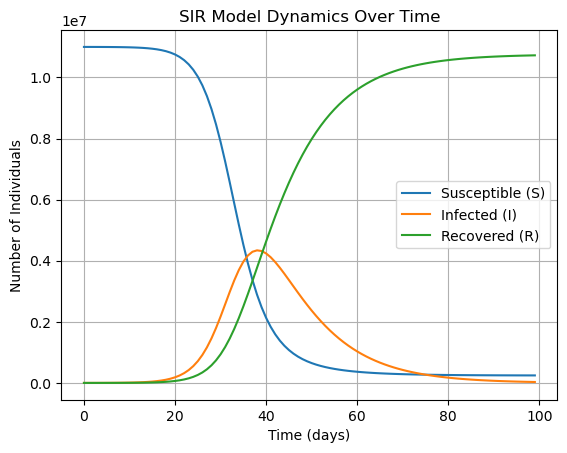
\includegraphics[width=0.8\textwidth]{sir_model_simulation.png}
\caption{Simulation of the SIR model showing the number of susceptible, infected, and recovered individuals over time.}
\end{figure}

\begin{figure}[h!]
\centering
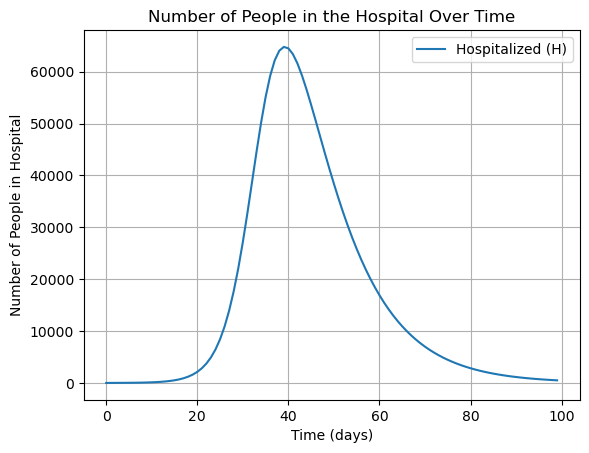
\includegraphics[width=0.8\textwidth]{hospitalization_dynamics.png}
\caption{Hospitalization dynamics over time, reflecting the average number of people in the hospital based on the rate of recoveries.}
\end{figure}

\section{Results and Discussion}
The simulation reveals the dynamics of disease spread and the impact of hospitalizations. The SIR model demonstrates how the number of susceptible, infected, and recovered individuals evolves over time. Incorporating hospitalization dynamics allows us to estimate the strain on healthcare systems. The figures show how the infection rate peaks before declining and how hospitalizations vary over time based on recovery rates.

\section{Conclusion}
This study extends the SIR model to include hospitalization dynamics, providing a more comprehensive view of epidemic progression. The Python implementation facilitates the analysis of complex epidemiological models and offers practical insights into disease management. Future research could explore additional factors such as varying hospitalization rates or different recovery durations.

\begin{thebibliography}{9}

\bibitem{SIRModel}
Kermack, W.O., and McKendrick, W. (1927). A Contribution to the Mathematical Theory of Epidemics. \textit{Proceedings of the Royal Society of London. Series A, Containing Papers of a Mathematical and Physical Character}, 115(772), 700-721.

\bibitem{COVIDData}
China CDC Weekly. (2020). COVID-19 Situation in Wuhan. \textit{China CDC Weekly}.

\bibitem{LukePolson}
Luke Polson,
\textit{Python Metaphysics Tutorials},
Unpublished.

\end{thebibliography}

\end{document}
